%%%%%%%%%%%%%%%%%%%%%%%%%%%%% BEGIN PACKAGE
\documentclass[11pt]{amsart}       % AMS template just for the draft
\usepackage{geometry}                 % See geometry.pdf to learn the layout options. There are lots.
\geometry{a4paper}                        % .letter or a4paper or a5paper or ... 
%\geometry{landscape}                 % Activate for for rotated page geometry
%\usepackage[parfill]{parskip}     % Activate to begin paragraphs with an empty line rather than an indent
\usepackage{graphicx}                   % FIgure
\usepackage{amssymb}                 % Math symbol
\usepackage{epstopdf}                   % for working in .pdf and  not .dvi (convert .eps, .jpg,  etc to .pdf)
\usepackage{psfrag}
\usepackage[T1]{fontenc}
\usepackage{aeguill}
\DeclareGraphicsRule{.tif}{png}{.png}{`convert #1 `dirname #1`/`basename #1 .tif`.png}
%%%%%%%%%%%%%%%%%%%%%%%%%%%%% END PACKAGE
\graphicspath{{PLOT/SinglePDGEMM/}}

%%%%%%%%%%%%%%%%%%%%%%%%%%%%% BEGIN AUTHORS AND INSTITUTIONS
\title{AMBIENT; an  execution and an MPI-CUDA scheduler  }
\author[A. Kosenkov, T. Ewart, B. Bauerb, A. Kantian,  M. Troyer, T. Giarmarchy]{Alexandr Kosenkov, Timoth\'ee Ewart, Bela Bauer, Adrian Kantian, Matthias Troyer and Thierry Giamarchy }
%\author[UNIGE, ETHZ, CSCS]{UNIGE, ETHZ, CSCS}
%%%%%%%%%%%%%%%%%%%%%%%%%%%%% BEGIN AUTHORS AND INSTITUTIONS


%%%%%%%%%%%%%%%%%%%%%%%%%%%%% BEGIN MACRO
\makeatletter
\newcommand\etc{\textit{etc}\@ifnextchar.{}{.\@}}
\newcommand\eg{\textit{e.g. }}
\newcommand\ie{\textit{i.e. }}
\newcommand\cf{\textit{c.f. }}

\makeatother
%%%%%%%%%%%%%%%%%%%%%%%%%%%%% END MACRO
\begin{document}

%%%%%%%%%%%%%%%%%%%%%%%%%%%%% BEGIN SYMBOL
\def\cloud{
\includegraphics[width=0.2cm]{FIGURES/cloud}}
%%%%%%%%%%%%%%%%%%%%%%%%%%%%% END SYMBOL
\maketitle

%%%%%%%%%%%%%%%%%%%%%%%%%%%%% BEGIN INTRODUCTION
\section{Introduction}

%Nowadays, the numerical simulations get an essential position, as experiments,  for studying physical 
%properties of many problems. The numerical simulations are presented inside every fields of sciences 
%and engineering, as classical and quantum mechanic, quantum chemistry,  \etc. As usual, the users always
%want increase the size of their problems, as billion number of particles for a kinetic simulation, billion 
%of meshes for a fluid dynamic computation, or else, matrixes of million entries for a quantum mechanic,
%or the linear algebra problems. Thus, the high performance computing is the solution for solving very large problem,
%with the peta flops  and the future generation of exa flops computers, the engineers and the scientists will
%have a quasi unlimited set of resources for modeling, nevertheless, they will be confronted to a challenge, have compatible
%programs for these machines. 

%A large set of programs; solvers, and software solutions are now availabled to solve large problem in a lot of fields, \eg we can 
%cite as popular in a few scientist field :  {\sc Quantum ESPRESSO} \cite{QE-2009} in quantum chemistry, Abinit \cite{ABINIT-2005, ABINIT-2009} in quantum mechanic,  ScaLAPACK \cite{SCALAPACK-1997} in linear 
%algebra,  or else SMILE in hypersonic rarefied flow \cite{SMILE-2005}. Of course, this short list is not exhaustive,
%and it can be fill up easily in every fields of science and engineering.

%If the scientists or the  engineers have the right tools, it will be necessarily  limited by the scalability of the code, in the case of the famous mathematical library ScaLAPACK, the
%efficiency  and thus the scalability, with the appropriated setting will reach up to 512 processors ($\sim  \mathcal{O}(100)$) \cite{SCALAPACK-1992}, beyond the interest is useless
%due to the degradation of the performance. In the worst case, the programmers will start  from a white page, and must design and efficient code.
%Due to the incredible number of cores, and optional accelerators as GPU, FGPA or "CELL like\footnote{Although the CELL processor is now depreciated, it herebies  
%a way of integrated processor (CPU+GPU), as the prove the last processor products of Intel (core i series) and AMD (fusion).}", the programmers 
%will have to introduce a mix programming model usually named mix-mode, based on a main MPI layer coupled with one or several additional layers \cite{EXASCALE-2010}.

%The most popular layer for mix-mode is OpenMP, and it is based on the preprocessor directives \texttt{\#pragma}, it demonstrated its performance. It is included successfully inside
%the  linear algebra libraries like the MKL from Intel or the PESSLSMP from IBM.  This ideology of the utilization of the pre-directives becomes more and more 
%important, thus it is used for vectorization of loops using the intel compiler and even for GPU with the PGI compiler. Although this ideology gives results, there is 
%a limitation for the main following reason: the creation/destruction of the threads will be extremely time consuming,
%when the  grain problem size becomes too fine \cite{SMITH-2001}. To achieve the best performance, the number of thread should be  equal to the number of cores on a socket, 
%thus the scalability will be increased at maximum by an order of magnitude.  The maximum number of processors now reach, becomes ($\sim \mathcal{O}(1000)$). 
%This ideology of implementation of the mix mode is more an evolution of the programming model than a revolution. It is an fast hand-on to implement that prolongates the life and the performance on a existing code. But,
%it will not prepare at all the code for the future, that will be automatically depreciated  by the new generation of cluster, in term of scalability.
   
%For getting several order of magnitude higher, we need a new programming model. The introduction of the GPU computing by NVidia a few years ago was
%a real innovation in HPC \cite{NICKOLLS-2010}. On a GPU, it is usual to program  thousand of threads. Thus, in this paper, we propose a innovative programming model to program on very large distributed cluster. We develop
%a framework named Ambient (C++) where we expend the CUDA programming ideology to  the a full cluster, thus we keep away the MPI programming model from the users.  In a way, we  extended
%the philosophy of OpenCL, OpenCL extents  the GPU programming model to a processor, assimilate a socket as a GPU, where every cores of the socket are assimilated to a streaming processor.
%We also developed inside a dynamic stack manager, that stocks and manages the execution of numerical "operations-solver" in functions of the resources of the distributed cluster.
   
%In this paper, we are going to describe our object oriented framework, and promote a first application based on linear algebra. Our main objective, is to 
%promote a new technology to develop  parallel application, without any interaction with the MPI and thread layer, and allow, a real access in term of performance to the next generation
%of clusters. The first possible  targets are applications that require large buffer of contiguous memory: quantum mechanic, linear algebra,  computational fluid dynamics, molecular dynamic \ldots 
%\, Until the end of this paper, we will focus on the linear algebra problems and their applications.


- Stress Performance of Ambient 
  - in terms of flexible and dynamical resource allocation
  - Stress performance boost derived from this (we need the benchmarks for that!)

%%%%%%%%%%%%%%%%%%%%%%%%%%%%% END INTRODUCTION

%%%%%%%%%%%%%%%%%%%%%%%%%%%%% BEGIN DESCRIPTION OF THE FRAMEWORK

\section{Design of the framework}
%In this section, we describe our framework in simple terms, without  a deep technical description.
%We will focus on the main functionalities  and show the essential features.

%%%%%%%%%%%%%%%%%%%%%%%%%%%%% BEGIN CUDA IDEOLOGY SECTION
\subsection{Extending the CUDA approach} \label{CUDAIDEOLOGYSECTION}

Ambient employs an extension on the CUDA approach to a distributed cluster. This is based on the observation that modern clusters employ many thousands of nodes, just like a GPU consists of thousands of small, simple cores, on each of which an runs an independent thread. In such a comparison however, the technical specifics of the basic cluster unit in terms of processor power, memory bandwidth, network speed, \etc  \, must be considered. 

The first thing coming in mind when we compare a  cluster and a GPU is the number of available cores.   Assimilate a single  CPU core  to  GPU core is reducer  because a CPU has additional capacities than a GPU core.
Thus, given the entirely different capabilities of a CPU core over a single GPU core, the scope of data for a single CPU (on which a single Ambient "thread" is typically running) in Ambient is rather comparable to that of a CUDA block or an OpenCL work group, the typical  blocks of size is $ 128 \times 128$. Of course, the user has full control of the size and can adapt it to the treated problem. Like in CUDA, blocks (i.e. groups of "threads") and a grid of blocks can then be formed in Ambient. A basic comparison between CUDA and Ambient is shown in the table \ref{ANALOGY}.

\begin{figure}[t]
	\begin{center}
	                  %psfrag for changing the layout
	                  \psfrag{New data layout}{\tiny{new layout}}
			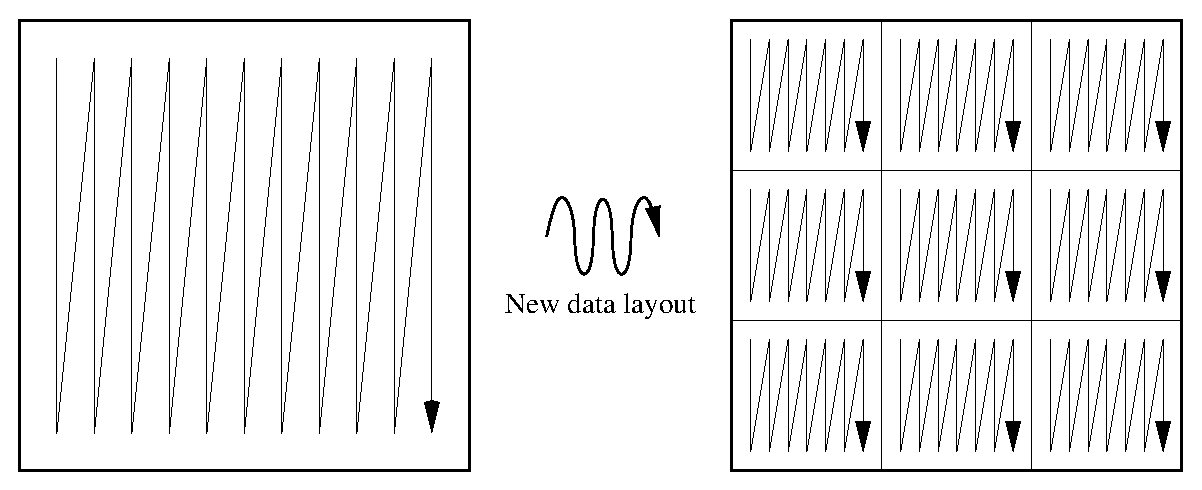
\includegraphics[scale=0.44]{FIGURES/MemMatrix.eps} 
	\end{center}
          \caption{Representation of the data layout inside the memory for linear algebra. We move from a single contiguous column data layout (left ) to several tile data layouts (right).}
          \label{MEMMATRIX}
\end{figure}

The work group approach imposes the adaptation of the data layout to the framework. In linear algebra,  BLAS \cite{LAWSON-1979} is \textit{de facto}  the standard for high performance dense Linear Algebra computations. It imposes column order on matrix storage, as well as a contiguous storage in memory (figure \ref{MEMMATRIX}).

For the sake of backward compatibility with the standard BLAS-based mathematical libraries (BLAS, LaPACK ScaLAPACK), we keep, the column order, but do not conserve a full contiguous buffer. As in the plasma library \cite{LTAIEF-2011}, we select
a tile data layout. It confers the ability to fit perfectly with the work group representation of Ambient, and further allows an excellent MPI/Thread control (section \ref{MPIABSTRACTION}). One of the main features of Ambient is to map this new data layout  to our work group approach, as shown in Fig. \ref{CUDAANALOGY}. 

\begin{table}[h]
	\begin{center}
	 	\begin{tabular}{c  c  c}
		 	                                                      & CUDA-OpenCL                                & Ambient            \\  \hline 
			 Device                                        & Graphic card/Processor (socket)   & Cluster               \\  
			  Entity  of Calculation               & GPU-Thread                                      & CPU-Thread     \\  
			 \begin{tabular}{c}
			 Scope of the \\ 
			 entity calculation  
                             \end{tabular}
                             &  Buffer entry                            & Full buffer \\
			 Execution model                       & Kernel                                                &  \begin{tabular}{c}  Logistic and \\ computational kernel   \end{tabular} \\
			 work group-ID                           &  \texttt{blockIdx}                                 & \texttt{get\_block\_id(A)}   \\  
			 work group size                        &  \texttt{blockDim}                               & \texttt{get\_dim\_id(A)}      \\  
			 grid size                                     &  \texttt{gridDim}                                  & \texttt{get\_grid\_dim(A)}  \\ \hline

		\end{tabular}
		\caption{Analogy between our framework and  the CUDA and OpenCL ideology.  \texttt{A} is the associated matrix to the  logistic and computational kernel.  
		The access of the cartesian values are done by the classical operator C/C++ \guillemotleft.\guillemotright     \, \eg \texttt{get\_dim\_id(A).x}  	\label{ANALOGY}}
	\end{center}
\end{table}

In CUDA and OpenCL, the execution model imposes kernel initialization with the appropriate resources (\eg numthread, numblock and grid dimension),
after which the user does not have to manage the memory access inside GPU memory; further, all threads can readily access any part of the GPU. Due to memory distribution in clusters we need to adapt this method of execution. Thus, we split this execution into two parts.

First, we prepare the memory, and then execute our "numerical" operation \eg a matrix multiplication in the following sequence \footnote{From here onwards, we will illustrate the execution model through parallel matrix addition and multiplication.}:
\begin{enumerate}
	\item A logistic kernel; where we select the number of processors, and map the memory with the datas.
	\item A computational kernel; where we execute the associated functions (the kernel in CUDA).
\end{enumerate}

\begin{figure}[!t]
	\begin{center}
           	        \psfrag{Ambient representation}{\tiny{\hspace{-0.4cm}Ambient representation}}
           	        \psfrag{CUDA/OpenCL representation}{\tiny{\hspace{-0.9cm}CUDA/OpenCL representation}}
	                 \psfrag{Associated mapping of the data with Ambient}{\tiny{\hspace{+0.15cm}Associated data mapping}}
	                 \psfrag{1x1 workgroup}{\tiny{\hspace{-0.5cm} \vspace{-0.1cm}1x1 workgroup}}
	                  \psfrag{of Ambient}{\tiny{\hspace{-0.4cm}\vspace{-0.9cm} of Ambient}}
	                  \psfrag{Workgroup of 4X4 threads}{\tiny{\hspace{-0.5cm} \vspace{-0.1cm}4x4 workgroup}}
	                  \psfrag{of CUDA}{\tiny{\hspace{-0.25cm}of CUDA}}
	                  \psfrag{Scope of GPU thread (left)}{\tiny{\hspace{-0.25cm}GPU scope left}}
	                  \psfrag{CPU (right)}{\tiny{\hspace{-0.7cm}CPU scope right}}       
		        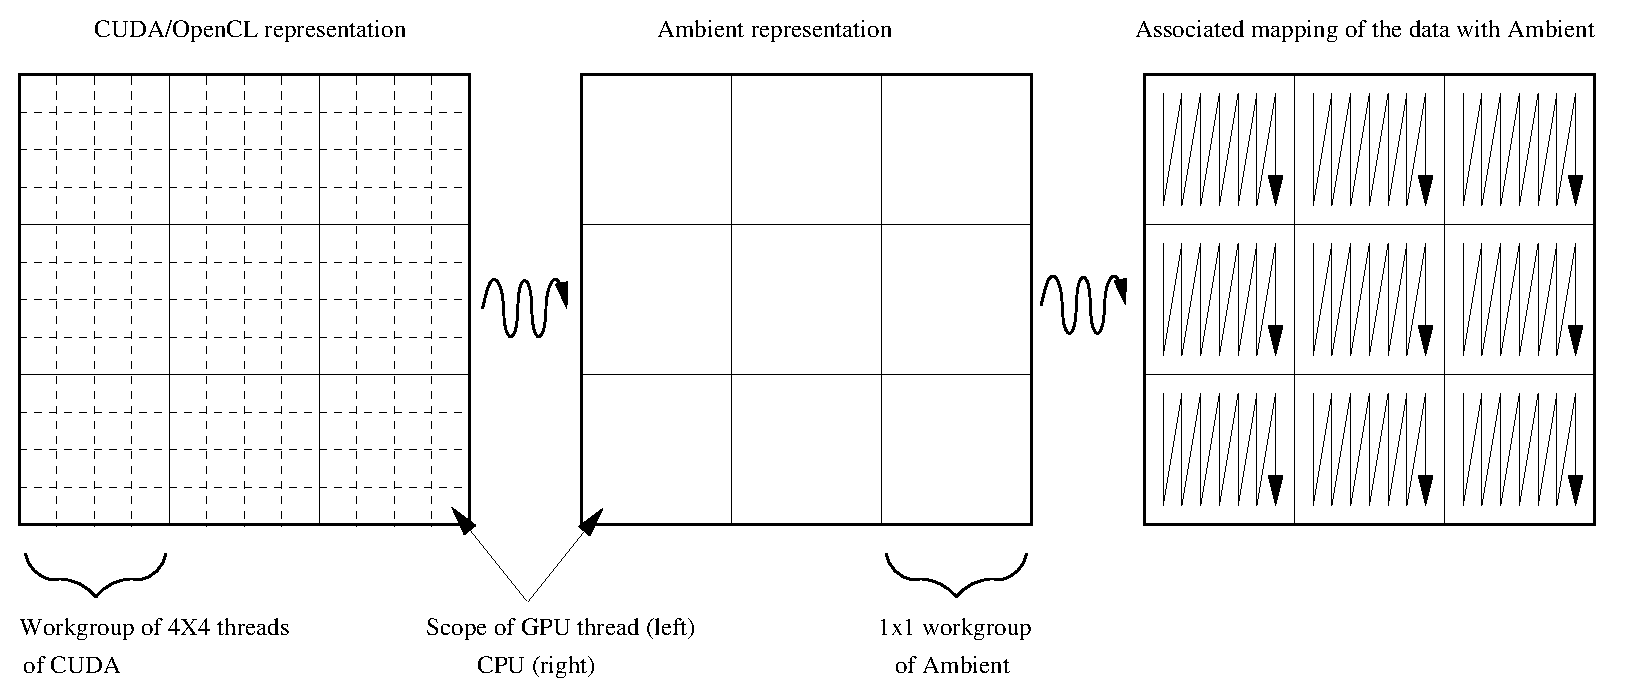
\includegraphics[scale=0.44]{FIGURES/CUDAanalogy.eps} 
	\end{center}
          \caption{Corresponding of the CUDA representation, to the ambient representation, in terms of the scope of the CPU with the associated data.}
          \label{CUDAANALOGY}
\end{figure}

Thus, every operations will have an associated logistics and computational kernel \eg multiplication, addition, or more sophisticated linear algebra operations

\subsubsection{The logistics kernel} The role of the logistics kernel is to initialize both memory and data for execution. It consists of creating a MPI-group and mapping the data to the group with the appropriate pattern (1D or 2D block-cyclic distribution for a matrix, or alternatively
a row/column-wise block distribution for two-dimensional Finite Difference Methods in fluid dynamics).  The creation of the group is done by an SQL-like request, and the data is mapped into this newly created group using a modular assignment
function. Both these functionalities are described in section \ref{SQLSECTION}.

In linear algebra, the optimal distribution in terms of load balancing is the 2D block-cyclic distributions, esp. in ScaLAPACK, but this will generally depend of the solver used. For example, in a QR factorization \cite{DEMMEL-2008} it can be demonstrated that a row-wise distribution is superior to a 2D block-cyclic decomposition for matrices with more rows than columns. Switching from one distribution scheme to another, which is a challenge in ScaLAPACK, is easily accomplished with Ambient.
 \begin{table}[t]  
	\begin{center}
	 	\begin{tabular}{l l }
                           \hline 
                           \textbf{Logistic kernel }  Algorithm of the addition logistics kernel  &    \\ \hline
                           \textbf{Require}                 A class Matrix  that fits with Ambient framework  &  \\
                           \begin{tabular}{c l} 
                           \tiny{1:} &  Addition\_logistic(Matrix $A$,  Matrix $B$)  \\
                           \tiny{2:} &  SQL request for selecting $N$ number of processors   \\
                           \tiny{3:} &  Perform 2/1-D cyclic distribution of the Matrix $A$  $\vartriangleright$ Note: the distribution \\
                                         & is performed with the number of processors selected inside the SQL request. \\
                           \tiny{4:} &  Perform 2/1-D cyclic distribution of the Matrix $B$ \\
%                           \tiny{5:} &  Perform 2/1-D cyclic distribution of the Matrix $C$ \\ 
                           \end{tabular} & \\ \hline
		 \end{tabular}  
		 \caption{Logistic kernel associated to the matrix multiplication or  the addition.  \label{LKERNEL}}
	\end{center}
\end{table}

To illustrate, we describe the example of a simplified\footnote{without any C++ language annotations} logistics kernel of the matrix addition in table {\ref{LKERNEL}}. 
\begin{itemize}
\item Line 1:  the signature of the logistics kernel, showing the input/ouput by the keyword\texttt{const}. In this example there are onlz three matrices, but additional arguments like float number, integer \etc can be added.
\item Line 2: The SQL-like request selecting the desired number of processors for the operation and performing the required MPI calls. 
\item Line 3-5: Performing a block-cyclic distribution of the matrixes \texttt{A} and  \texttt{B}. A detailed description of the SQL requests and the distribution functions
is given in section \ref{SQLSECTION}. Note that the present kernel can be reused for any subsequent operation that uses the same data distribution.
\end{itemize}

\subsubsection{The computational kernel}  After the logistics kernel has been executed, we are ready for the computational kernel. The mode of execution is similar to the CUDA API with a few specificities. In the CUDA parallel computing model, the programmer writes a single thread program, using the CUDA-API,  after which the GPU runs multiple instances of this thread in parallel. We transpose this approach into Ambient. Nevertheless, we should not forget the data scope of a single CPU "thread" in Ambient roughly corresponds to the scope of a full OpenCL work group. 

We have introduced a keyword (as the \texttt{const} keyword) named \texttt{pinned}. This keyword indicates to the framework than the kernel execution must be executed over all Ambient work groups. Inside a kernel, we employ several Ambient API, analogous to CUDA, to obtain key information about the work groups 
(positions, dimensions, \ldots).These are summarized in table \ref{ANALOGY}.  For illustration, the computational kernel (table \ref{CKERNEL}) of an addition of the two matrices associated with the previous example of the logistics kernel is presented in the table \ref{LKERNEL}.
\begin{itemize}
\item Line 1: the signature of the computational kernel must be the same than that of the associated logistics kernel. The only difference is the use of the keyword \texttt{pinned}, indicating an execution over all Ambient work groups.
\item Line 2: the cartesian coordinates of the work group are obtained from the Ambient instruction \texttt{get\_block\_id(A).x}  for $i$ and \texttt{get\_block\_id(A).y}  for $j$. \label{CURRENT}
\item Line 3 to 5 : we refer the work group $i,j$ to a temporary variable $A_{ref}$ using the Ambient instruction \texttt{current(A)(i,j)}. Note that if the processor requires data outside its memory, it will perform a remote access in the background (see section ... for details).
\item Line 6 to 8 : the addition is performed by looping over the total size of the work group, in parallel for each workgroup (because of the use of the keyword \texttt{pinned}.
\end{itemize}

 \begin{table}[t] 
	\begin{center}
	 	\begin{tabular}{l l }
                           \hline 
                           \textbf{Computatiomal kernel }  Algorithm of the addition computational kernel  &    \\ \hline
                           \textbf{Require}                 A class Matrix  that fits with Ambient framework  &  \\
                           \begin{tabular}{c l} 
                               \tiny{1:} &  Addition\_computational(Matrix $A$,  \texttt{pinned const}  Matrix $B$) \\
                               \tiny{2:} &  Get the cartesian coordinate $i,j$ of the work group \\ 
                               \tiny{3:} &  Refer  the  work group$(i,j)$  of A into $A_{ref}$ \\
                               \tiny{4:} &  Refer  the  work group$(i,j)$  of B into $B_{ref}$ \\
%                               \tiny{5:} &  Refer  the  work group$(i,j)$  of C into $C_{ref}$  \\
                               \tiny{5:} &  \textbf{for} $k$ from $0$ to total size of the work group \textbf{do} \\
                               \tiny{6:} & \hspace{0.2 cm}   $A_{ref}[k] \, + \!\! = B_{ref}[k]$ \\
                               \tiny{7:} &  \textbf{end for} \\                               
                          \end{tabular} & \\ \hline
		 \end{tabular} 
		 \caption{Algorithm of the computational kernel associated to the matrix addition.   \label{CKERNEL}}
	\end{center}
\end{table} 

As just shown for the matrix addition, we can recode other linear algebra solvers with the Ambient approach. For the presentation of our framework, we will focus on the MPI version of BLAS named pBLAS \cite{SCALAPACK-1992}, as well as a possible alternative to the pDGEMM solver, called ...., using a recursive algorithm.

%\begin{table}[h]
%	\begin{center}
%	 	\begin{tabular}{c  c  c}		 	                                                             & CUDA/OpenCL                                 & Ambient                               \\  \hline 
%			 work group-ID                                  &  \texttt{blockIdx}                                 & \texttt{get\_block\_id(A)}   \\  
%			 work group size                               &  \texttt{blockDim}                               & \texttt{get\_dim\_id(A)}      \\  
%			 grid size                                            &  \texttt{gridDim}                                  & \texttt{get\_grid\_dim(A)}  \\ \hline
%				\end{tabular}
%		\caption{Analog�y between Ambient and  the CUDA/OpenCL ideology. \texttt{A} is the associated matrix to the present logistic and computational kernel.  The access of the cartesian values are done by the classical operator C/C++ \guillemotleft.\guillemotright     \, \eg \texttt{get\_dim\_id(A).x}  } 	
%		\label{ANALOGY2}
%	\end{center}
%\end{table}


%%%%%%%%%%%%%%%%%%%%%%%%%%%%% END CUDA IDEOLOGY SECTION

%%%%%%%%%%%%%%%%%%%%%%%%%%%%% BEGIN SQL SECTION

\subsection{SQL resource management}  \label{SQLSECTION}
 In the previous section, we introduced the logistics kernels and their role in initializing resources for the execution of the computational kernels. 
 One of Ambients' main qualities is the ability to perform a dynamic management of the CPU resources of the cluster. To facilitate this, we integrated a light SQL framework [cite something] inside Ambient, which selects the desired number of processors inside the logistics kernel, in order to execute the computational kernel. 

At the beginning of the framework execution, a main MPI group is created named \texttt{ambient}. To create groups inside this main group we used the abilities of MPI to build nested independent groups of processors  (chapter 6 of  \cite{MPI-2002}).  We encapsulated these features in the framework, and we control them through the SQL requests. This allows for a simple yet flexible management  of the MPI groups.  
These requests (done by the \texttt{scope\_select} Ambient-function) are applied to the logistics/computational addition kernels of our example by the following SQL syntax: \\

\begin{eqnarray}
       & &\texttt{scope\_select("\textit{N} from ambient as addition\_group }   \label{SQL1} \\
       & &\texttt{	where master is 0")}, \nonumber
\end{eqnarray}
This command selects \texttt{\textit{N}} processors from the original MPI group  \texttt{ambient}. The newly created group is 
named \texttt{addition\_group}, and its master processor locally has MPI-rank 0 (see Fig. \ref{MPIGROUP}).

\begin{figure}[h]
	\begin{center}
           	         \psfrag{Datas distributed over work group}{\tiny{\hspace{-0.5cm}Datas distributed over work group}}
	                  \psfrag{Local MPI rank}{\tiny{Local MPI rank}}                
	                  \psfrag{Ambient master proc}{\hspace{-0.8cm} \tiny{Ambient master proc}}        	                  
	                   \psfrag{Ambient MPI group, N process}{ \tiny Ambient MPI group, cardinal $N$ process}
	                   \psfrag{Local rank}{\tiny Local rank}
	         	         \psfrag{0}{\tiny{0}}
	                  \psfrag{1}{\hspace{-0.05cm}\tiny{1}}
	                  \psfrag{2}{\hspace{-0.15cm} \tiny{2}}
	                  \psfrag{MPI group creation}{ \hspace{-0.5cm} \tiny  Group creation}
	                  \psfrag{from the SQL request}{ \hspace{-0.6cm} \tiny  from SQL request}
	                  \psfrag{Mapping of the work group throw}{ \hspace{-0.6cm} \tiny  Mapping of the work group throw}
	                  \psfrag{the mpi GROUP created}{\tiny the new MPI group}
	                 \psfrag{(0,0)}{\hspace{-0.25cm} \tiny (0,0)}
	                 \psfrag{(0,1)}{\hspace{-0.25cm} \tiny (0,1)}
		        \psfrag{(0,2)}{\hspace{-0.25cm} \tiny (0,2)}
		        \psfrag{(1,0)}{\hspace{-0.25cm} \tiny (1,0)}
		        \psfrag{(1,1)}{\hspace{-0.25cm} \tiny (1,1)}
		        \psfrag{(1,2)}{\hspace{-0.25cm} \tiny (1,2)}
	                 \psfrag{(2,0)}{\hspace{-0.25cm} \tiny (2,0)}
		        \psfrag{(2,1)}{\hspace{-0.25cm} \tiny (2,1)}
		         \psfrag{(2,2)}{\hspace{-0.25cm} \tiny(2,2)}
                           \psfrag{n}{\hspace{-0.25cm} \tiny $n$}
	                  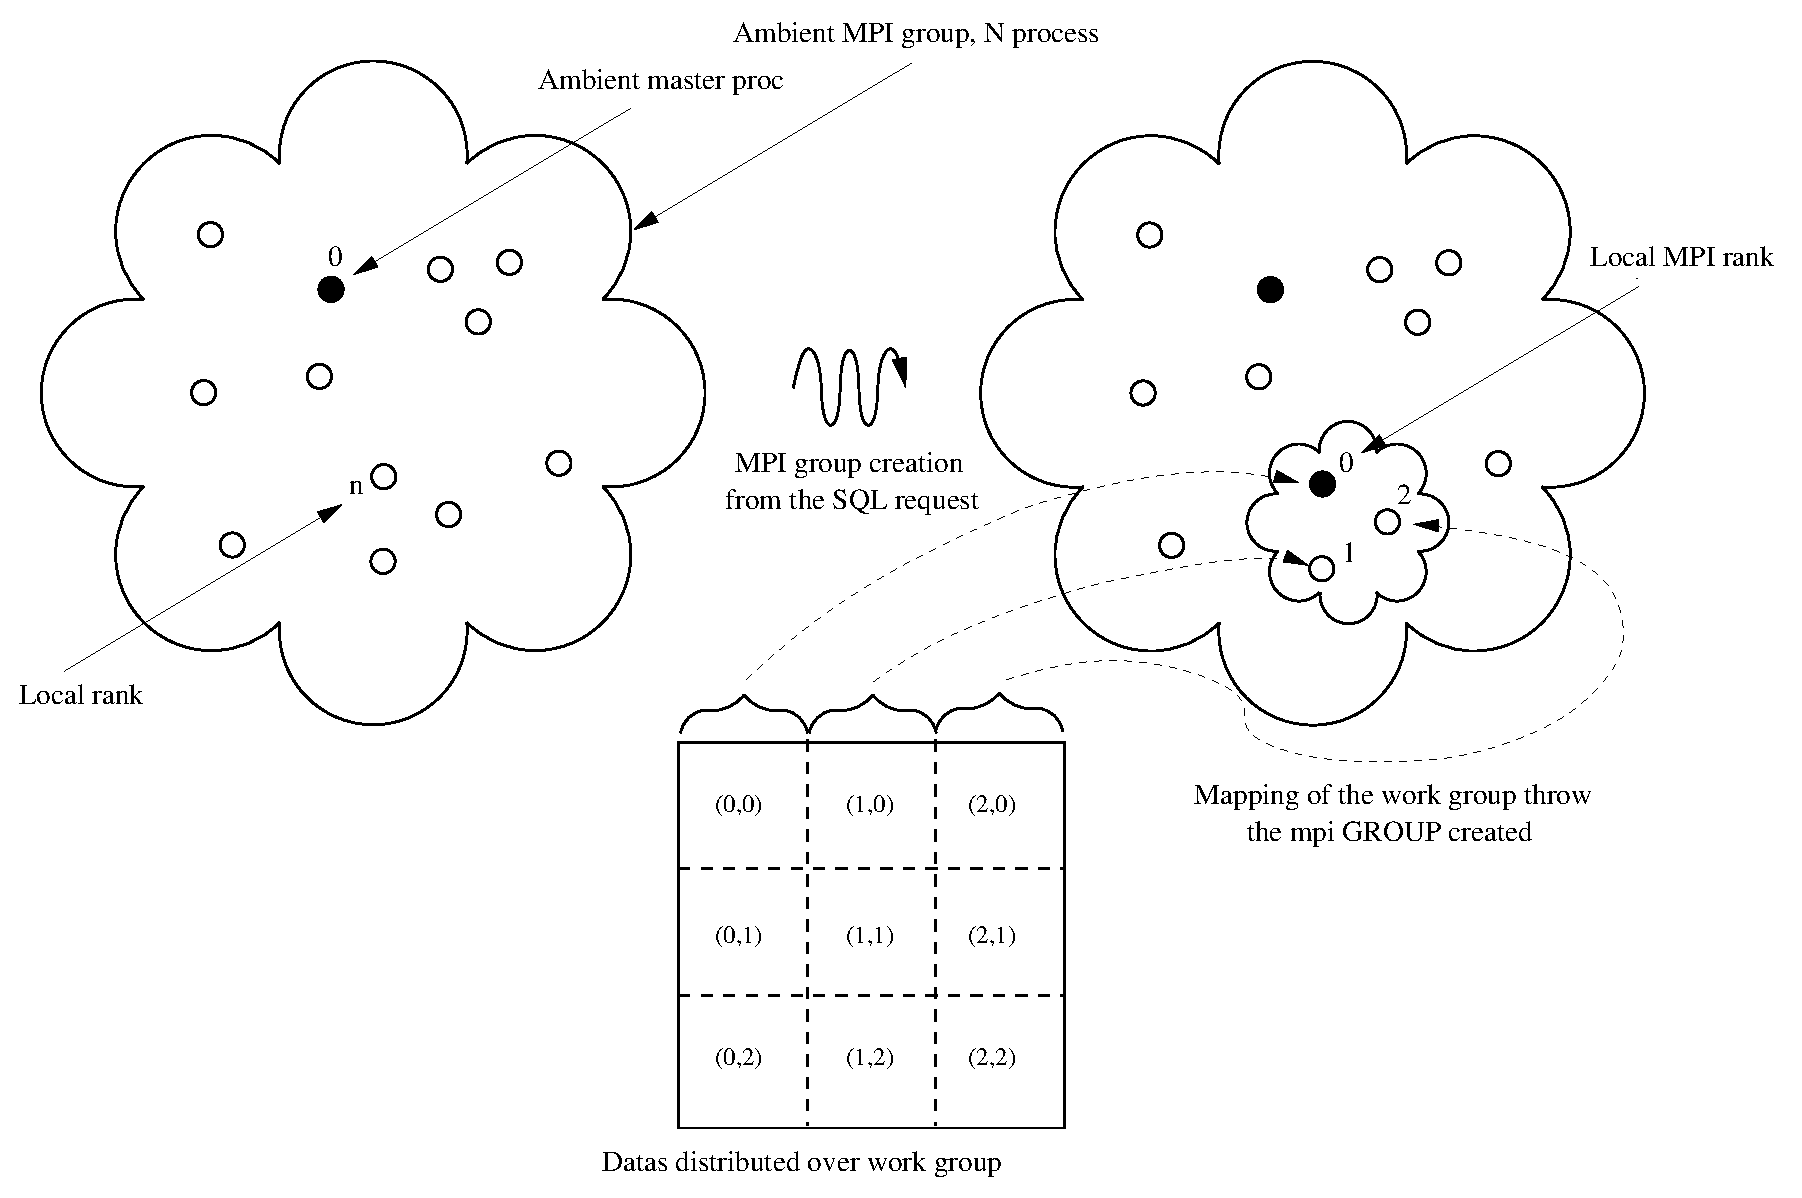
\includegraphics[scale=0.35]{FIGURES/MpiGroupData.eps} 
	\end{center}
          \caption[]{Creation of a MPI group by the SQL request, with \hbox{\cloud \hspace{0.02cm}} representing a MPI group with its own communicator;  $\bullet$ represents the master 
          process inside the group whereas the $\circ$ are the associated slave processors inside the corresponding group. Also shown is the assignment of the data blocks (each block corresponding to an Ambient work group) inside the newly created MPI group. In this example, the matrix is mapped, block by block, on the processors using a 1D column-cyclic distribution.}
          \label{MPIGROUP}
\end{figure}

After the SQL request, the data (workgroup) is mapped to the processes inside the newly created MPI group by a distribution function (\eg 1D or 2D block-cyclic distribution), the algorithm of which is described in table \ref{2DCYCLIC} (\cf Fig. \ref{MPIGROUP}). After this transfer, the processes of the MPI group are the primary owners in terms of data access and execution. In the Ambient approach, every operation is associated with
a logistics and a computational kernel, therefore the SQL request will be called several times. To create new groups, processes from the existing group are selected in ascending numerical rank, until all processes of the \texttt{ambient} group 
have been selected. If further groups are required, the selection is restarted from the beginning, thus a processor can belong to multiple groups simultaneously.

Every new group will have its own intra-communicator to allow intra-group communication, as well as an inter-communicator to allow for communication between groups, using the master process of the \texttt{ambient} group.

The construction of nested MPI-groups is related to the ability of MPI to create virtual and cartesian topologies  (chapter 7 of  \cite{MPI-2002}). However, Ambient allows for the simultaneous construction of the MPI topology and the mapping of the  data (work group).

 \begin{table}[t] 
	\begin{center}
	 	\begin{tabular}{l l }
                           \hline 
                           \textbf{Assign workgroup}  Algorithm of the 1/2-D assign function  &    \\ \hline
                           \textbf{Require}        An new MPI group obtained by an SQL request  &  \\
                           \begin{tabular}{c l} 
                               \tiny{1:} &  Initialize $i$ in function of the new MPI rank  of the new group \\
                               \tiny{2:} &  Initialize $j$ in function of the new MPI rank  of the new group  $\vartriangleright$ Note:   \\
                                             &  the initialization of $i,j$ will fix   the distribution (1D or 2D) \\
                               \tiny{3:} &  \textbf{for} from $i$  to the number of the work group on $x$ \textbf{do} \\
                               \tiny{4:} &  \hspace{0.2 cm}  \textbf{for} from $j$  to the number of the work group on $y$ \textbf{do} \\
                               \tiny{5:} & \hspace{0.4 cm}    Assign the work group $(i,j)$ to the corresponding processor\\
                               \tiny{6:} &   \hspace{0.2 cm}    \textbf{end for} \\
                               \tiny{7:} &  \textbf{end for} \\                               
                          \end{tabular} & \\ \hline
		 \end{tabular} 
		 \caption{Algorithm of the distribution of the work group into the new MPI group.   \label{2DCYCLIC}}
	\end{center}
\end{table} 

During the execution, many group will be created in practice, and data will have to be moved between groups.
To obtain better performance and to reduce the number of data transfers between groups, there are additional possible settings for the SQL request. For example, consider the previous illustration for the SQL request in case of the matrix addition operation ($ A \, +\!\!\!= B$).
If matrix $A$ has already been created and mapped on specific processors, the logistics kernel can create a MPI group that includes its previous owner group (created in the previous operation), thereby avoiding superfluous data transfer. The concrete SQL request would be as follows:
 
\begin{eqnarray}  \label{SQL2}
         & & \texttt{scope\_select("\textit{N} from ambient as addition\_group }\\ 
         & & \texttt{	where master is 0 where breakdown contains" + get\_id(\textit{A})}, \nonumber
\end{eqnarray} 
The function \texttt{get\_id(\textit{A})} will get a tag  of \texttt{\textit{A}} to know is present binding.
 
%\begin{figure}[h]
%	\begin{center}
%			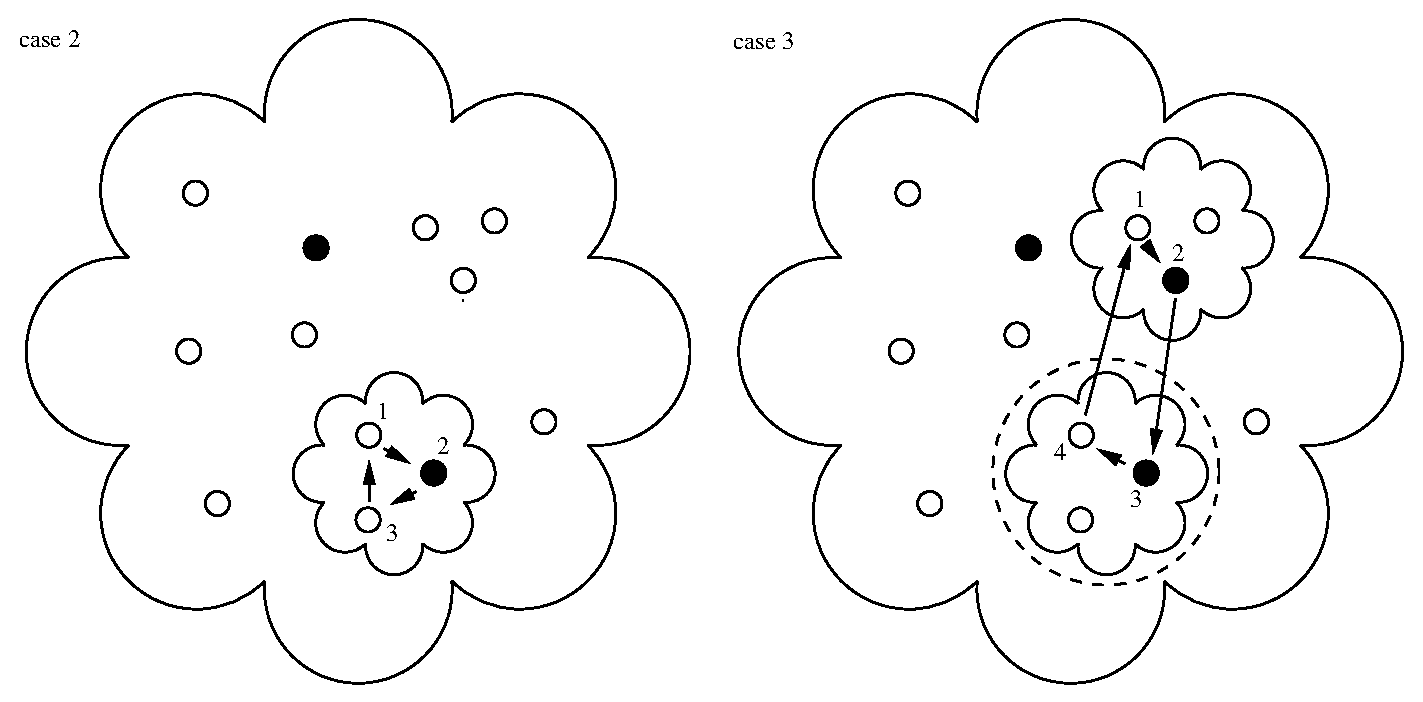
\includegraphics[scale=0.35]{FIGURES/ComGroup.eps} 
%	\end{center}
%          \caption{Data exchange inside the group.}
%          \label{COMGROUP}
%\end{figure}

%%%%%%%%%%%%%%%%%%%%%%%%%%%%% END SQL SECTION

%%%%%%%%%%%%%%%%%%%%%%%%%%%%% BEGINNING EXECUTION AND OPERATIONS SCHEDULING SECTION
\subsection{Execution model and Operations scheduling}
In a typical HPC application, the programming model imposes a parallel execution of every function of the code, step by step, where the data granularity
of the problem  has imposed the parallelization. In ambient, we developed an scheduler, an  \guillemotleft engine\guillemotright \, that privileged a queue execution model  (promoted  and popularized by the CELL processor), where operations (\eg linear algebra operations \ldots)
will be stacked up into a list  and then executing according the model of logistics/computation kernel. This model is inspired from computer architecture design;
the queue data flow execution in a processor \cite{DENNIS-1974}, nevertheless, we are working now on a larger scale where basic instructions ($+,-,*,/$) are  replaced 
by the pair logistics/computation kernels. 

An HPC application can be always decomposed as a set of functions that perform numerical operations.  Start by a basic example, we want to perform the three following algebra operations :

\begin{eqnarray} 
\text{Operation 1:} & & A + \!\! =  B, \label{3OPERATIONS}  \\
\text{Operation 2:} & & A \times \!\!= 3,   \nonumber  \\ 
\text{Operation 3:} & & C \times \!\!= D. \nonumber
\end{eqnarray}

In the usual way, the three operations will be executed in parallel one after one. Transposing this example in Ambient's conception means; each operation is now  associated to a logistics and a computational kernel. In Practice, considering our addition example(\ref{3OPERATIONS}),  the users will use the following \texttt{push} function:

\begin{eqnarray}
     \texttt{push(Addition\_logistics, Addition\_computional, \textit{A}, \textit{B})},
\end{eqnarray} 

where we have the appropriated logistics and computational kernel named \texttt{Addition\_logistics} and \texttt{Addition\_computational}  presented in the table \ref{LKERNEL} and \ref{CKERNEL} previously, followed by the two arguments \texttt{\textit{A}} and \texttt{\textit{B}}. During the execution of the application, operations will be stack up, and in an ideal case, the content of the stack should be executed at the end of the application. Nevertheless, the users have the possibility to execute the content of the stack during the code,
by the basic following instruction :

\begin{eqnarray}
      \texttt{playout().}
\end{eqnarray} 

This command triggered on the engine of ambient. The engine will scan through the stack of operation and identifies the independent operations, and also mark the different dependencies by incrementing a local dedicated counter. Then, it adds a  dedicated MPI packet manager\footnote{A packet manager is a tool that manages the communication between processors.} (see section \ref{MPIABSTRACTION})  for every operations and performed all logistics kernels. Due to the dependencies, the data will be map in a first MPI group and marked as need in others, with a trace of the previous owner.
Finally, the independent computational kernels are executed followed by  the depending computational kernels in the appropriated order. In case of dependency of the data, the migration of the datas will be done by the packet manager. 
When all computational kernels are over, the stack is cleaned. Thus, this method combined to the execution of the computational kernels creates two layers of parallelization : the simultaneous execution of  kernels executed in parallel.  
A schematic of the stack execution is presented on Fig. \ref{EXECUTION} 

\begin{figure}[h]
	\begin{center}
	      	        \psfrag{Operation 1}{\tiny{Operation 1}}
		        \psfrag{Operation 2}{\tiny{Operation 2}}
		        \psfrag{Operation 3}{\tiny{Operation 3}}
		        \psfrag{l/c kernel 1}{\tiny{l/c kernel 1}}
                           \psfrag{l/c kernel 2}{\tiny{l/c kernel 2}}
                           \psfrag{l/c kernel 3}{\tiny{l/c kernel 3}}
                           \psfrag{Abiemt}{\tiny{Ambient}}
                           \psfrag{schedule}{\tiny{Schedule}}
                           \psfrag{Dependency}{\tiny{Dependency}}
                           \psfrag{Time}{\tiny{Time}}
                           \psfrag{evolution}{\tiny{evolution}}
                           \psfrag{Mapping and execution}{\tiny{Mapping and execution}}                          
                           \psfrag{Ambient execution}{\tiny{Ambient execution}}                          
                           \psfrag{Usual execution}{\tiny{Usual execution}}                          
	                  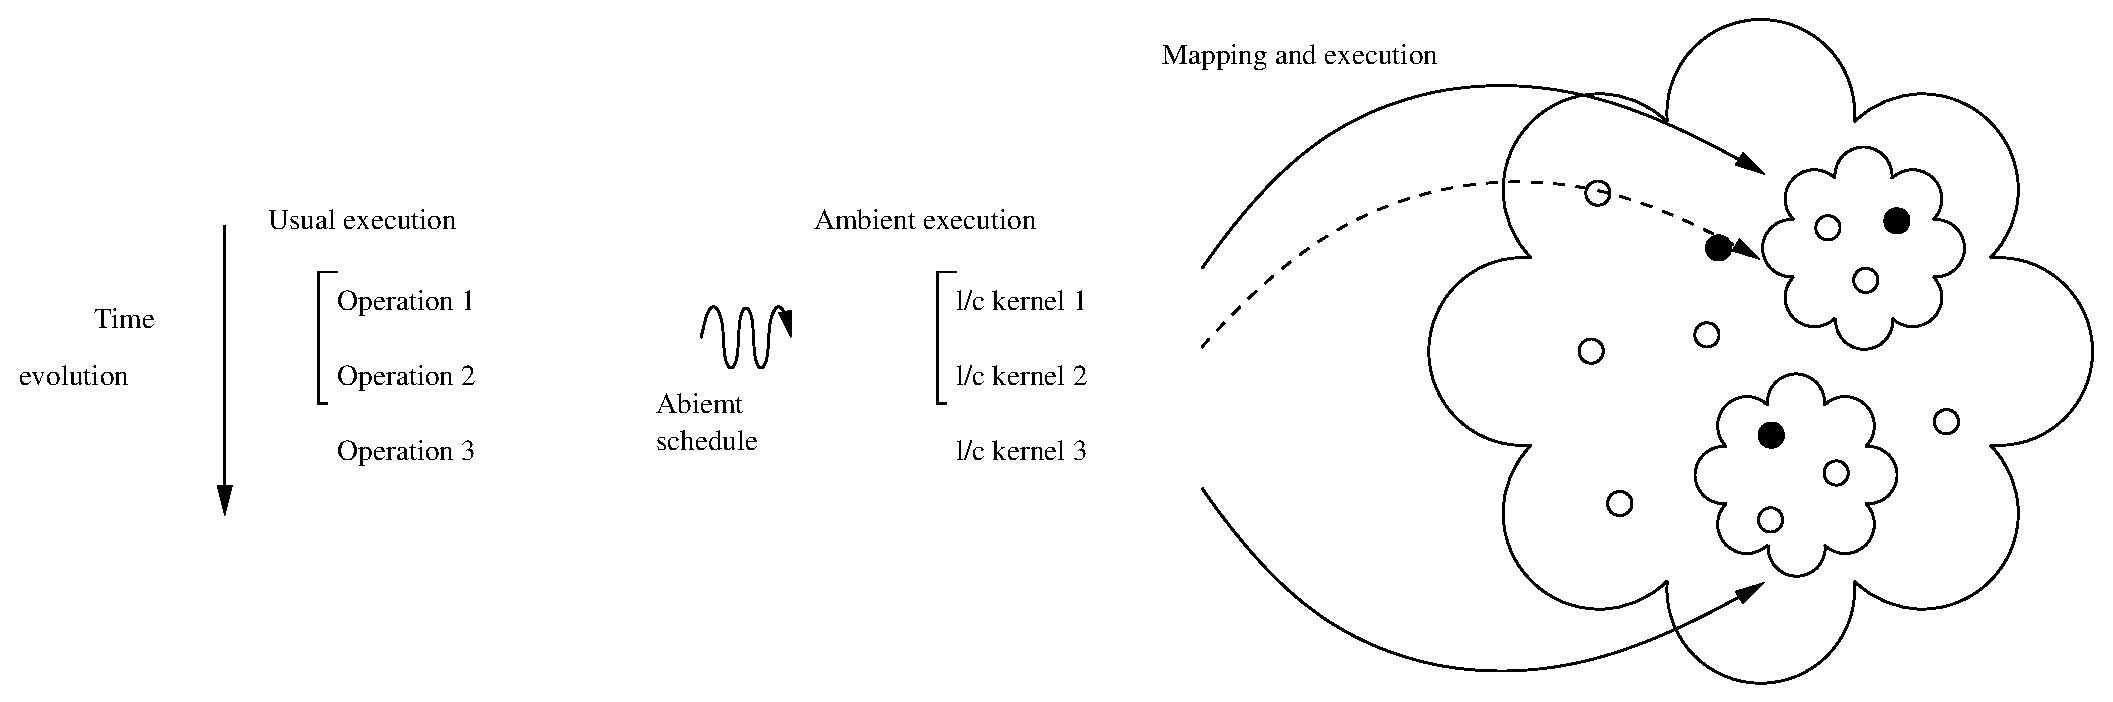
\includegraphics[scale=0.35]{FIGURES/execution.eps} 
	\end{center}
          \caption{Model of execution of the ambient scheduler. On the classical approach (left) the operations will be executed in parallel step by step whatever the dependencies (marked by the symbol \guillemotleft [\guillemotright \, in the schematic). In ambient (right), operations will be associated to the pair logistics/computation (abbreviate l/c) kernel, as operations 1 and 3  (l/c kernels 1 and 3) are independents, the execution of computational kernel will be done, simultaneously.  Due to the dependency between the kernel 1 and 2, the computational kernel of operation 2 (l/c kernel 2) will be executed later. It should be performed in a new MPI group but  with an appropriate SQL request (\ref{SQL2}) in logistics kernel, we can execute the computational kernel where the data are. }   \label{EXECUTION}
\end{figure}

Now, we  generalized the example \ref{3OPERATIONS} to a vectors of matrices. We  add  conditional statements to know which matrices should add and multiply (Table \ref{GRAPH}). First, from line 1 to 11, as a dry run, the application execution will determine which operations should be performed, 
and it will pushed up needed kernels on the top of stack. When the \texttt{playout()} function is called line 12, the engine will execute the stack, by solving dependency, it will  create the directed  acyclic graph of the application, naturally. Moreover this example shows the strength of Ambient, we have integrated a double parallelization without any, hard coding of MPI instruction in the original code. Thus, a full parallel linear algebra  application can be developed without taking into account the geometry of the problem, which usually done.

\begin{table}[t] 
	\begin{center}
	 	\begin{tabular}{l l }
                           \hline 
                           Determination of the directed  acyclic graph   &    \\ \hline
                           \textbf{Require}    A class Matrix  that fits with Ambient framework   &  \\  
                           and  vector of matrices  of size $n$, $A[n]$, $B[n]$, $C[n]$ and $D[n]$ & \\
                           \begin{tabular}{c l} 
                               \tiny{1:}   & \textbf{for} from $i$  to the size of the vector \textbf{do} \\
                               \tiny{2:}   & \hspace{0.2 cm} \textbf{for} from $j$  to the size of the vector \textbf{do} \\                               
                               \tiny{3:}   & \hspace{0.4 cm}  \textbf{if}  the conditions on $A[i]$ and  $B[j]$ are verified \textbf{do} \\                               
                               \tiny{4:}   & \hspace{0.8 cm}  $A[i]+ \!\! =B[j]$, $\vartriangleright$  push l/c kernel 1, \\
                               \tiny{5:}   & \hspace{0.4 cm} \textbf{end if} \\   
                               \tiny{6:}   & \hspace{0.4 cm} $A[i]\times \!\! =3$,  $\vartriangleright$  push l/c kernel 2, \\                   
                               \tiny{7:}   & \hspace{0.4 cm} \textbf{if}  the conditions on $C[i]$ and  $D[j]$ are verified \textbf{do} \\                               
                               \tiny{8:}   & \hspace{0.8 cm} $C[i]\times \!\! =D[j]$,  $\vartriangleright$ push l/c kernel 3, \\
                               \tiny{9:}   & \hspace{0.4 cm}  \textbf{end if} \\       
                               \tiny{10:} & \hspace{0.2 cm}  \textbf{end do} \\   
                               \tiny{11:} & \textbf{end do} \\                                 
                               \tiny{12:} & \texttt{playout()} $\vartriangleright$  execute the stack \\
                               \tiny{13:} & $\vartriangleright$ Note:  $+\!\!=$ and $\times \!\! =$ operators have wrapper functions   \\
                                                & that push the good logistics and computational kernel. \\                               
                           \end{tabular}   &  \\ \hline
        	     \end{tabular}
	\end{center}
	\caption{Generalization of the example \ref{3OPERATIONS} with conditional statements. The association of a cumulative stack and  delate stack execution will determine the  directed  acyclic graph. \label{GRAPH}}
\end{table} 

To conclude this section, unlike a typical parallel execution, this model have several decisive advantages. It allows a transparent parallelization of two layers of parallel execution, and most important, it determined the directed  acyclic graph on the full application in order to get the best performance.


%%%%%%%%%%%%%%%%%%%%%%%%%%%%% END EXECUTION AND OPERATIONS SCHEDULING SECTION

\subsection{Packet manager and MPI abstraction} \label{MPIABSTRACTION}
In a normal HPC application, the  data could be prepared when communications are needed, if the data have more than one type especially. In this case  
we should prepare a MPI structure and then perform the exchange. These preliminary conversions are painful for the performance. In  Ambient,
 the structure of data layout by work groups necessitates additional metadata to coordinate the good executions of logistics and 
 computational kernels. Particularly, when a remote access is performed in 
a computational kernel. Thus,  before the block of data (literally the numbers 
inside the matrix) of the any workgroups,  contiguous data  are included. We called this ensemble \guillemotleft block of data+metadata\guillemotright \, as a netweork packet. It is built
on a MPI structure. Thus the work groups  are  ready to send or receive without any additional movements or copying. 
To assure the good execution of the framework, several additional type of packets are  available, they all derived from a standard packet. 
%The control of the packet and MPI exchange is done by a packet manager.

When we execute a computational kernel, we get the data by the Ambient command  \texttt{current(\textit{A})(i,j)} (ref. \ref{CURRENT}), where \textit{A} is a matrix 
compatible with Ambient, and the indices $i$ and $j$ are the coordinates of the work group (Fig. \ref{MPIGROUP}). Three possibilities are possibles for getting the data when a process execute this functions
in a computational kernel.
\begin{enumerate}
\item The work group is already in the memory of the process. The access is direct.
\item The work group is in the memory space of the present MPI-group (previously created by the associated logistics kernel). The applicant process sends a query request (a specific packet) to its  master process of its MPI group.
The master process of the group gets the request (the master process knows the repartition of the workgroup inside the MPI-group), it sends a new request to
the actual owner, when the actual owner gets the request, it send the workgroup needed to the first applicant. 
\item The work group is inside an other MPI-group. As previously, the applicant process sends to the master process a query  request, and the master process of 
the actual MPI group  sends an other request to the older owner group. The older master process gets the message and sends a message to actual owner of the data. Then the owner 
of the data sends the data to the first applicant.
\end{enumerate}
We illustrate the two last previous situations on the figure \ref{MPIEXCHANGE}.
\begin{figure}[h]
	\begin{center}
	    \psfrag{case 2}{\tiny case 2}
	    \psfrag{case 3}{\tiny case 3}
             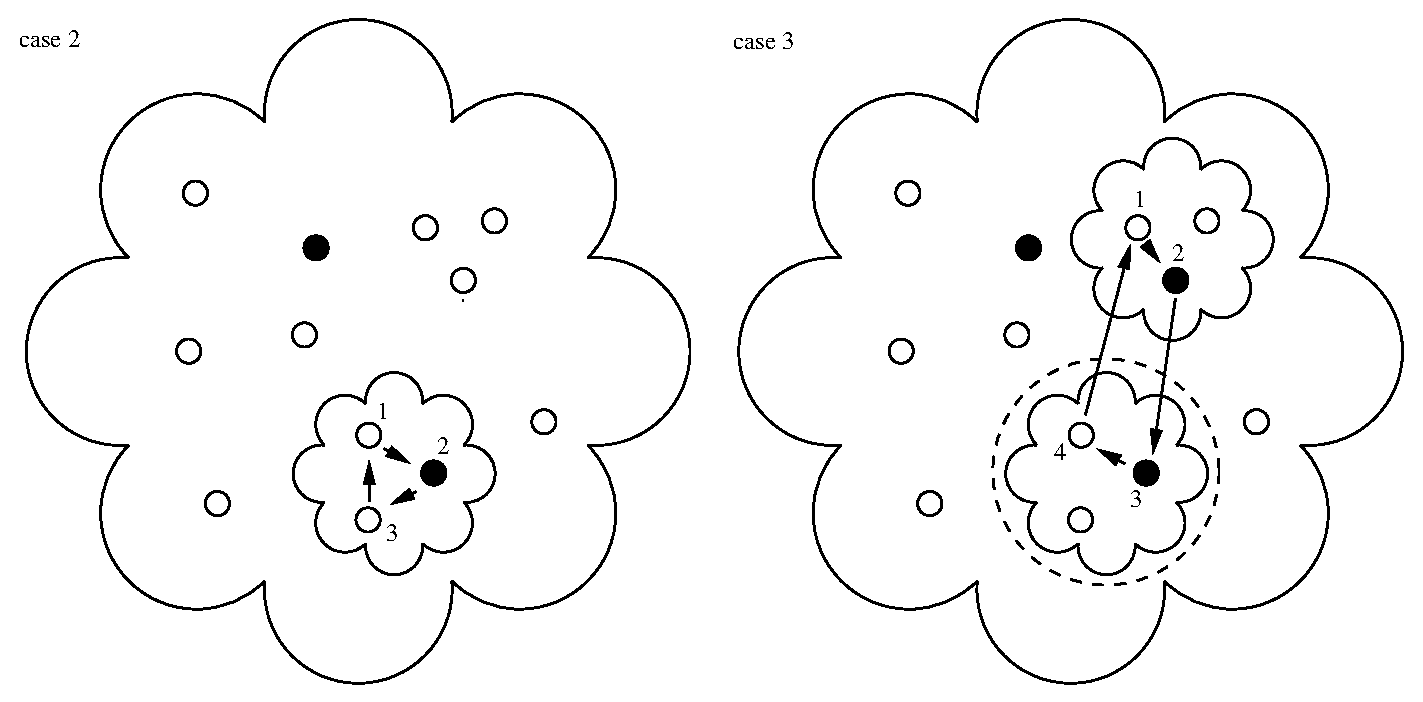
\includegraphics[scale=0.35]{FIGURES/ComGroup.eps} 
	\end{center}
          \caption{On the left, we illustrate communications inside the same group. On the right, we illustrate the communications between  two MPI-groups. The dashed circle indicated the previous MPI group. In both cases, the masters process have the key 
          role to distribute informations for the exchange. The requests  are arrows, and the orders of operations are marked by numbers.}  \label{MPIEXCHANGE}
\end{figure}

In the previous section, we reveled the importance of the communications, theirs perfect execution is relevant to  the packet manager.
The packet manager  manages the intra communication inside the same MPI group \eg to perform an multiplication, and the inter communication
between the MPI groups. The packet manager is unique for every MPI-group, it is based on a singleton pattern. 


 In the previous paragraph, we presented different communication blueprint when datas are requested by a process.
As communication path between the applicant  and the owner of the data can be more and less complex,  to solve every communication scheme,  we designed the packet manager on two main things :
the delegate pattern and a finite state machine (FSM).

To reach the best performance in HPC,  synchronization operations should be avoided  \cite{EXASCALE-2010}, because it is  a bottleneck.
Thus, we privileged  MPI asynchronous communication into Ambient (\texttt{mpi\_isend} and \texttt{mpi\_irecv}). Nevertheless, if a message 
is sent by a asynchronous instruction, an MPI test is necessary to check if the packet can be received.  As we refused synchronization instructions,
we repeat the process until receiving the message by an infinite loop. Thus we integrated the delegate pattern and the FSM inside the loop.


\begin{table}[t] 
	\begin{center}
	 	\begin{tabular}{l l }
                           \hline 
                           Algorithm of the packet manager   &    \\ \hline
                           \textbf{Require}  a MPI process require a block of data &  \\                           
                            \begin{tabular}{c l}                                
                               \tiny{1:}   & \textbf{for}  ;;  \textbf{do} $\vartriangleright$  infinite loop \\
                               \tiny{2:}   & \hspace{0.2 cm}  \texttt{Delegate()}  $\vartriangleright$ check if  packet has been, \\
                                                & and received and re-send if needed \\
                               \tiny{3:}   & \hspace{0.2 cm}  FSM $\vartriangleright$ break the loop, \\
                                               & if all packets arrived at destination. \\
                               \tiny{4:}   & \textbf{end do} \\
                           \end{tabular}   &  \\ \hline
        	     \end{tabular}
	\end{center}
	\caption{Description of the packet manager}
\end{table} 



\begin{figure}[h]
	\begin{center}
	    \psfrag{1}{\tiny \hspace{-0.1 cm}  1}
	    \psfrag{2}{\tiny \hspace{-0.1 cm}  2}
	    \psfrag{Loose}{\tiny \hspace{-0.2 cm}   Loose}
	    \psfrag{Closure}{\tiny \hspace{-0.2 cm}  Closure}
	    \psfrag{Open}{\tiny \hspace{-0.4 cm}  Opening}
             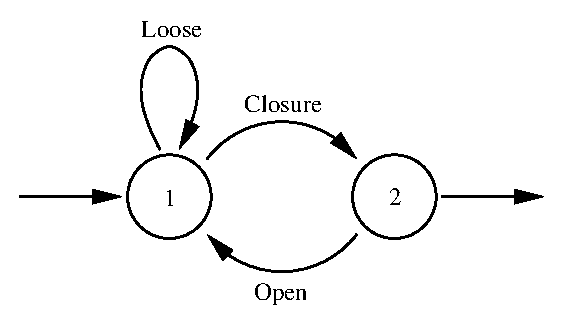
\includegraphics[scale=0.45]{FIGURES/FSM.eps} 
	\end{center}
          \caption{Schematic of the finite sate machine for the closing procedure. The states 1 and 2 correspond to open or close. The transitions are loose, closure or opening, they  depend of the situation of all packets (if they all reach theirs targets or not),
                          the loose transition means the packet has not been received, thus we iterate one more time on the infinite loop.}  \label{FSM}
\end{figure}



A delegate pattern (C\#) encapsulated methods,    It is similar to pointer of function under C++  but is allows a safer execution, we ported this pattern into Ambient.
The packet manager class contains a delegate object. The delegate class contains a series of operations pill-up  in a stack. These operations consists of forwarding requests, 
 block of data,  layout of the MPI group (block distribution) and theirs updates. As this delegate is included, into an infinite loop, the packets
will propagate process by process after every iterations (as shown on Fig. \ref{EXECUTION}). At the end of the delegate execution, a finite state machine checks the states of the packets. 
If all packets received (data packet, layout packet, \ldots), the FSM (Fig. \ref{FSM}) breaks the infinite loop.


\subsection{Abstract parallel datatypes} % <- to change ? 

\subsection{Validation}
As  validation test, we code a new implementation of PDGEMM using our framework, and we compare to the classical version of PDGEMM of ScaLAPACK (MKL-Version).
The algorithm of our implementation is based on the classical method using a columns order distribution for the matrices nevertheless, we give a description of the algorithm 
into the table \ref{AMBIENTDGEMM} to show the modification due to Ambient. 



The main advantages in our implementation is the size of coding, it is limited at 7 lines  of code using our framework.

----------------------------------------------------------------------------------------------------- \\
TO DO EXPLAIN THE ADVANTAGE AGAINST   SCALAPACK \\
IN TERM OF NETWORK, DATA EXCHANGE \\
----------------------------------------------------------------------------------------------------- \\

The results will be compare with the ScaLAPACK implementation, in the section \ref{CUDAIDEOLOGYSECTION}, we announced a compatibility with the ScaLAPACK.
The representation of the memory of ScaLAPACK and Ambient have significant differences, although matrixes are subdivided into small block, the layout into
the memory is different. In Ambient all blocks named work group are independent even if they belong to the same process. In ScaLAPACK block will be regrouped
by process to get a contiguous memory, the multiplication between blocks will be assure by using a correct offset inside the DEGMM call. Therefore, in ambient if we execute a solver from ScaLAPACK,
one of the first operation to perform will be the rearrangement of the work groups of a same owner into a contiguous block. This operation add a certain overload.

 \begin{table}[t] 
	\begin{center}
	 	\begin{tabular}{l l }
                           \hline 
                           \textbf{ Algorithm:}  pDGEMM using Ambient  &    \\ \hline
                           \textbf{Require}                 A pinned computational kernel  &  \\
                           \begin{tabular}{c l} 
                                 \tiny{1:} &  Get the cartesian coordinate $i,j$ of the work group \\ 
                                 \tiny{2:} &  Refer  the  work group$(i,j)$  of B into $B_{ref}$ \\
                                 \tiny{3:} &  \textbf{for} from $k(0)$  to the max number of rows \textbf{do} \\
                                 \tiny{4:} &  \hspace{0.2 cm} Refer  the  work group$(k,j)$  of A into $A_{ref}$ \\    
                                 \tiny{5:} &  \hspace{0.2 cm}  reduction of the blocks $(k,i)$ into $C_{ref}$ , $\vartriangleright$  The reduction, \\
                                                & \hspace{0.2 cm}  is done by a proxy pattern \\
                                 \tiny{6:} &  \hspace{0.2 cm}  classical DGEMM($A_{ref}$, $B_{ref}$, $C_{ref}$)\\
                                 \tiny{7:} &  \textbf{end do} \\    
                             \end{tabular} & \\ \hline
		 \end{tabular} 
		 \caption{Algorithm of the pDGEMM using Ambient framework. We remember a proxy pattern is an interface the something else (object in memory). There, it allows the reduction between the independent workgroups.   \label{AMBIENTDGEMM}}
	\end{center}
\end{table} 



The validation test consists of multiplying matrices and saving the results into an output matrix, as follow :
\begin{eqnarray}
C = A \times B
\end{eqnarray}
This test will be executed with the ambient computational kernel and the Scalapack PDGEMM solver inside Ambient (with the additional workload of rearrangement of the memory)
As we are using C++ language, the operations $\times$ and $=$ have been overloaded correctly by pushing the good logistics and computational kernels.
When the calculation is over for both methods results are compared element by element respecting the following test  \cite{Dongarra:1990:SLB:77626.79170} :

\begin{eqnarray}
\frac{\left \lvert C^S_{ij} - C^A_{ij} \right \rvert}{\left \lvert  \epsilon C^S_{ij} \right \rvert } < n,
\end{eqnarray}

Where  the precision factor $\epsilon$  is equal to the \texttt{double} precision $10^{-16}$, the indices  $S$ and $A$ represent the ScaLAPACK and the Ambient version,
indices $i$ and $j$ are the entries of the matrices and $n$ is equal to 16 (decimal digits), the exponent of the numerical precision. 

For the validation the size of work groups have been fixed to $128 \times 128$, and the matrices are squares from 256 up to 8196 (by step of 128 elements). The numbers of MPI-Process varied from 2 to 8.
Matrices were filled up with pseudo random number generator  \texttt{drand48()}\footnote{This function returns 
pseudo-random numbers non-negative, double-precision,  uniformly distributed over the interval $[0.0 , 1.0]$ using a linear congruential algorithm and 
48-bit integer arithmetic. }  from \texttt{stdlib}.  The validation tests have always been verified successfully . The benchmarks are performed and evaluated in the next sections.

%%%%%%%%%%%%%%%%%%%%%%%%%%%%% END DESCRIPTION OF THE FRAMEWORK


\section{Results and discutions}
\subsection{First benchmark case}
The first benchmark consists of evaluating the performance of our parallel matrix multiplication. The initial condition are the same than the validation test. The benchmarks 
were performed on a AMD-2427 2.2 Ghz ..........

\begin{figure}
% GNUPLOT: LaTeX picture with Postscript
\begingroup
  \makeatletter
  \providecommand\color[2][]{%
    \GenericError{(gnuplot) \space\space\space\@spaces}{%
      Package color not loaded in conjunction with
      terminal option `colourtext'%
    }{See the gnuplot documentation for explanation.%
    }{Either use 'blacktext' in gnuplot or load the package
      color.sty in LaTeX.}%
    \renewcommand\color[2][]{}%
  }%
  \providecommand\includegraphics[2][]{%
    \GenericError{(gnuplot) \space\space\space\@spaces}{%
      Package graphicx or graphics not loaded%
    }{See the gnuplot documentation for explanation.%
    }{The gnuplot epslatex terminal needs graphicx.sty or graphics.sty.}%
    \renewcommand\includegraphics[2][]{}%
  }%
  \providecommand\rotatebox[2]{#2}%
  \@ifundefined{ifGPcolor}{%
    \newif\ifGPcolor
    \GPcolorfalse
  }{}%
  \@ifundefined{ifGPblacktext}{%
    \newif\ifGPblacktext
    \GPblacktexttrue
  }{}%
  % define a \g@addto@macro without @ in the name:
  \let\gplgaddtomacro\g@addto@macro
  % define empty templates for all commands taking text:
  \gdef\gplbacktext{}%
  \gdef\gplfronttext{}%
  \makeatother
  \ifGPblacktext
    % no textcolor at all
    \def\colorrgb#1{}%
    \def\colorgray#1{}%
  \else
    % gray or color?
    \ifGPcolor
      \def\colorrgb#1{\color[rgb]{#1}}%
      \def\colorgray#1{\color[gray]{#1}}%
      \expandafter\def\csname LTw\endcsname{\color{white}}%
      \expandafter\def\csname LTb\endcsname{\color{black}}%
      \expandafter\def\csname LTa\endcsname{\color{black}}%
      \expandafter\def\csname LT0\endcsname{\color[rgb]{1,0,0}}%
      \expandafter\def\csname LT1\endcsname{\color[rgb]{0,1,0}}%
      \expandafter\def\csname LT2\endcsname{\color[rgb]{0,0,1}}%
      \expandafter\def\csname LT3\endcsname{\color[rgb]{1,0,1}}%
      \expandafter\def\csname LT4\endcsname{\color[rgb]{0,1,1}}%
      \expandafter\def\csname LT5\endcsname{\color[rgb]{1,1,0}}%
      \expandafter\def\csname LT6\endcsname{\color[rgb]{0,0,0}}%
      \expandafter\def\csname LT7\endcsname{\color[rgb]{1,0.3,0}}%
      \expandafter\def\csname LT8\endcsname{\color[rgb]{0.5,0.5,0.5}}%
    \else
      % gray
      \def\colorrgb#1{\color{black}}%
      \def\colorgray#1{\color[gray]{#1}}%
      \expandafter\def\csname LTw\endcsname{\color{white}}%
      \expandafter\def\csname LTb\endcsname{\color{black}}%
      \expandafter\def\csname LTa\endcsname{\color{black}}%
      \expandafter\def\csname LT0\endcsname{\color{black}}%
      \expandafter\def\csname LT1\endcsname{\color{black}}%
      \expandafter\def\csname LT2\endcsname{\color{black}}%
      \expandafter\def\csname LT3\endcsname{\color{black}}%
      \expandafter\def\csname LT4\endcsname{\color{black}}%
      \expandafter\def\csname LT5\endcsname{\color{black}}%
      \expandafter\def\csname LT6\endcsname{\color{black}}%
      \expandafter\def\csname LT7\endcsname{\color{black}}%
      \expandafter\def\csname LT8\endcsname{\color{black}}%
    \fi
  \fi
  \setlength{\unitlength}{0.0500bp}%
  \begin{picture}(7200.00,4536.00)%
    \gplgaddtomacro\gplbacktext{%
      \csname LTb\endcsname%
      \put(814,704){\makebox(0,0)[r]{\strut{} 0}}%
      \put(814,1299){\makebox(0,0)[r]{\strut{} 5}}%
      \put(814,1893){\makebox(0,0)[r]{\strut{} 10}}%
      \put(814,2488){\makebox(0,0)[r]{\strut{} 15}}%
      \put(814,3082){\makebox(0,0)[r]{\strut{} 20}}%
      \put(814,3677){\makebox(0,0)[r]{\strut{} 25}}%
      \put(814,4271){\makebox(0,0)[r]{\strut{} 30}}%
      \put(1513,484){\makebox(0,0){\strut{} 1024}}%
      \put(2269,484){\makebox(0,0){\strut{} 2048}}%
      \put(3024,484){\makebox(0,0){\strut{} 3072}}%
      \put(3780,484){\makebox(0,0){\strut{} 4096}}%
      \put(4536,484){\makebox(0,0){\strut{} 5120}}%
      \put(5292,484){\makebox(0,0){\strut{} 6144}}%
      \put(6047,484){\makebox(0,0){\strut{} 7168}}%
      \put(6803,484){\makebox(0,0){\strut{} 8192}}%
      \put(176,2487){\rotatebox{-270}{\makebox(0,0){\strut{}GFlops}}}%
      \put(3874,154){\makebox(0,0){\strut{}Matrix size}}%
    }%
    \gplgaddtomacro\gplfronttext{%
      \csname LTb\endcsname%
      \put(5816,4098){\makebox(0,0)[r]{\strut{}Peak}}%
      \csname LTb\endcsname%
      \put(5816,3878){\makebox(0,0)[r]{\strut{}pDGEMM ScaLAPACK}}%
      \csname LTb\endcsname%
      \put(5816,3658){\makebox(0,0)[r]{\strut{}pDGEMM Ambient}}%
    }%
    \gplbacktext
    \put(0,0){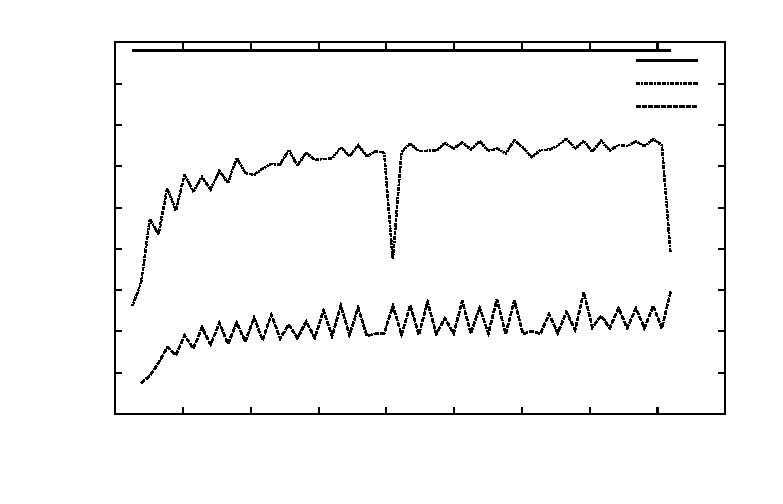
\includegraphics{SinglePGEMM}}%
    \gplfronttext
  \end{picture}%
\endgroup

\end{figure}


\subsection{Second benchmark case}
\subsection{Third benchmark case}

\section{Conclusions}

%%%%%%%%%%%%%%%%%%%%%%%%%%%%% BEGIN BIBLIO
\bibliographystyle{abbrv}
\bibliography{biblio}
%%%%%%%%%%%%%%%%%%%%%%%%%%%%% END BIBLIOr



\end{document}  